\chapter{绪论}

在大数据时代,每天都会产生海量的数据,涵盖各个领域,例如电子商务平台、社交网络、医疗健康等。二分图 (Bipartite Graph) 作为有效的数据表示方法,能准确描述两个不同群体间的关系,比如电子商务中用户与商品的购买关系,因此被广泛应用于数据建模和分析。其中,极大二分团是二分图中稠密子图,代表两个紧密连接的群体。通过枚举极大二分团,我们可以发现和理解数据中的信息,对知识挖掘、数据分析和智能决策等方面至关重要。因此,极大二分团枚举 (Maximal Biclique Enumeration, MBE) 问题备受研究领域关注。本文从剪枝技术、数据结构和并行实现三种角度出发,研究大规模二分图场景下高效的极大二分团枚举方法,并对应形成三种独立的解决方案。接下来,本章将依次介绍本文的研究背景、研究课题、国内外研究现状、研究挑战以及本文的研究内容和组织结构。

% 本文主要研究课题是大规模二分图中的极大二分团枚举方法。本章介绍了本课题研究背景,国内外研究现状以及本文的研究内容和组织结构。

\section{研究背景}

随着信息技术的迅猛发展和广泛应用,人类社会正逐渐进入大数据时代,大规模数据的生成和积累已成为一种常态。这些数据涵盖了生活的方方面面,并蕴藏着丰富而有价值的信息。为了充分挖掘和利用这些数据中所蕴含的有效信息,二分图结构被广泛应用于表示两个不同群体之间的联系~\cite{bipartite22}。在\emph{二分图}中,顶点 (Vertex) 代表着不同的数据实体,而边 (Edge) 则表示实体之间的关系。二分图结构能够清晰地描述出数据实体之间的交互和连接。具体而言,在二分图中,顶点被划分为两个不同的集合,而同一集合内的顶点之间并未直接相连。例如,在如图\ref{fig:eg_intro}所示的电子商务的场景下,二分图描绘了用户和商品之间的关系,其中顶点可以表示用户或商品,而边则表示购买关系。二分图可以很好地描述了用户与商品之间的关联行为。此外,\emph{二分团}是指在二分图中形成的一种稠密子图,它代表着数据集中那些紧密连接的群体。以电子商务为例,二分团可以表示同一群用户对同一组商品的产生的批量购买行为。这种紧密的连接揭示了数据中存在的某种规律或者共同特征,为理解群体交易行为提供了一定的线索。而\emph{极大二分团}是指在二分图中那些独立于其他所有二分团的特殊二分团。它们具有独立性和独特性,不被其他任何二分团所完全包含。\textbf{识别并枚举二分图中的极大二分团,有助于发现更为细致和确切的群体信息,进一步为深入探究群体行为内部的脉络和联系提供帮助。}

\begin{figure} [ht]
  \centering
  \vspace{0.05in}
  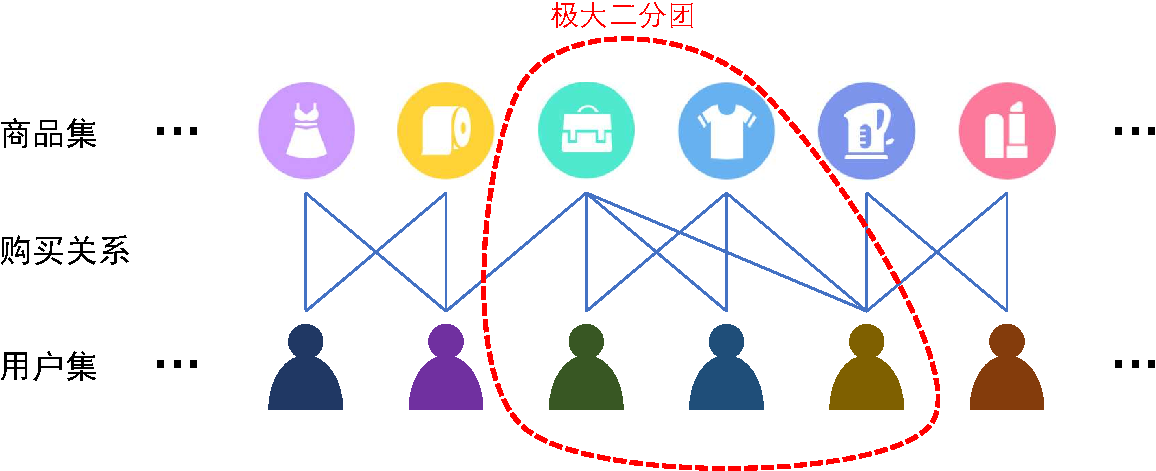
\includegraphics[width=0.7\linewidth]{eg_intro}
  \vspace{0.05in}
  \caption{电子商务场景下的二分图与极大二分团}
  \label{fig:eg_intro}
\end{figure}



% 极大二分团枚举在二分图\textbf{数据挖掘}方面起到重要辅助作用,具有广泛的应用价值。
\textbf{极大二分团枚举在数据挖掘领域具有广泛的应用价值。} (1) 在电子商务场景下,极大二分团被广泛应用于描述用户群体对同一组商品的批量购买行为。电子商务领域的领军企业如阿里巴巴、eBay和亚马逊通常使用二分图表示"用户----购买----商品"的交易关系~\cite{MEB20}。一些不法商家会利用刷单手段,雇佣一批用户购买目标商品,以提高其曝光率并扰乱市场秩序。考虑到极大二分团能有效描绘此类刷单行为,电子商务企业可以通过枚举极大二分团来发现所有可疑交易,提升对刷单行为的检测率~\cite{clickfarm21,MEB20,MEB22,skylinechinese23}。(2) 在社交网络场景下,极大二分团最大程度地描述了用户群体的相同兴趣爱好。通过极大二分团枚举,可以更好地辅助社交推荐系统。通过发现用户之间紧密的连接关系,系统可以推荐给用户其他拥有相似兴趣爱好的用户,从而增加社交互动和用户满意度。同时,极大二分团的枚举还能帮助社交网络平台理解用户行为和需求,进一步优化用户体验,提高平台的粘性和竞争力~\cite{minel06,MBEchinese17}。同时,通过极大二分团的枚举,还有助于对社交网络进行全面分析,有助于发现社交网络中存在的异常风险信息,提升社交网络安全防护工作的能力~\cite{dangerous19,dangerous05}。(3) 在基因分析场景下,极大二分团描述了同一组基因对同一组性状的决定作用。枚举极大二分团能够更好地帮助生物学家理解基因与性状之间的关系。通过分析不同基因之间的连接模式,可以揭示基因之间的相互作用以及它们对性状表现的综合影响。这种基于极大二分团的分析方法能够提供更全面和深入的基因功能研究视角,帮助科学家进一步进行蛋白质-蛋白质相互作用网络分析~\cite{protein11}、从事务数据库中提取基因表型信息~\cite{gene11}、构建最优进化树~\cite{tree04}以及探索基因表达机制~\cite{geneexp11}。此外,极大二分团的枚举还有助于准确预测基因变异对性状造成的影响,并为疾病研究、遗传工程等领域提供重要的指导意义~\cite{gene22,iMBEA14,protein21}。(4)在图神经网络 (Graph Neural Network, GNN) 领域,极大二分团能够辅助对多个节点数据进行打包,从而加速GNN信息聚合。通过识别和利用极大二分团结构,可以将具有相似特征或者相互关联的节点分为同一个二分团,更高效地进行信息传递和计算,提升图神经网络的训练和推理性能~\cite{Pqbiclique21,Pqbiclique23,Pq23}。总而言之,极大二分团的枚举在电子商务、社交网络、基因分析以及图神经网络等领域都发挥着重要的作用。它能够帮助揭示群体行为、发现异常的交易行为、辅助推荐系统和加速信息聚合等任务,为相关领域的研究和实践提供有力支持。

\begin{figure} [t]
  \centering
  \vspace{0.1in}
  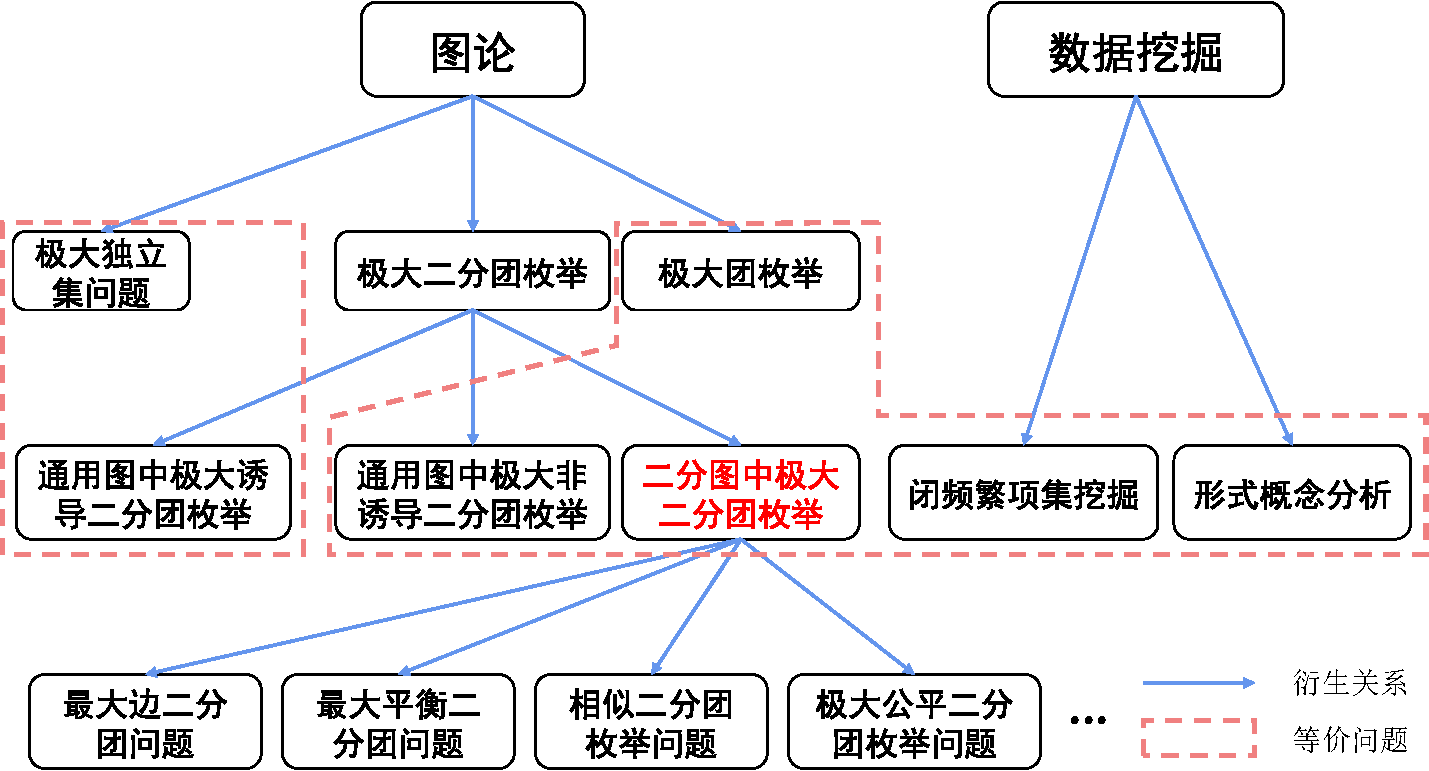
\includegraphics[width=0.9\linewidth]{directory}
  \vspace{0.1in}
  \caption{二分图中极大二分团枚举问题与相关问题的关系图}
  \label{fig:directory}
\end{figure}

\textbf{同时,极大二分团枚举也是图论中的一类经典组合优化问题。}
% 同时,二分图中的极大二分团枚举问题作为\textbf{图论}中的经典组合优化问题,吸引了广泛的研究兴趣。
下面,我们结合图~\ref{fig:directory},从三个方面(相近问题、等价问题和衍生问题)介绍本研究问题与其他相关问题的联系。(1)相近问题:极大二分团是一种特殊的子图,在通用图中同样存在。通用图中的极大诱导二分团枚举问题可转化为极大独立集问题进行求解~\cite{MBE-induced21};通用图中的极大非诱导二分团枚举问题可转化为二分图中的极大二分团枚举问题进行求解~\cite{Proof09}。考虑到二分图中的极大二分团枚举问题具有广泛的应用价值,本文仅研究二分图中的极大二分团枚举问题。(2)等价问题:二分图中的极大二分团枚举问题与许多图论领域和数据挖掘领域的经典问题存在一一映射关系。例如,极大团枚举问题~\cite{MCEchinese17,MCE20,MCEchinese20,MCE-GPU21,MCEchinese21,MCE22,MCEreview22} (Maximal Clique Enumeration, MCE)、闭频繁项集挖掘问题~\cite{FCIM98,FCIM22} (Frequent Closed Itemset Mining, FCIM) 和形式概念分析问题~\cite{FCA21,FCA22} (Formal Concept Analysis, FCA)。很多现有的极大二分团枚举方法都受益于这些相关问题的优化思路,部分相关工作将极大二分团枚举问题规约到这些相关问题进行求解。我们将在第~\ref{sec:related}节详细介绍这些方法。相应地,对二分图中极大二分团枚举问题的优化研究间接地为解决这些问题提供了思路。(3)衍生问题:随着二分图中极大二分团问题研究的深入,近年来,极大二分团枚举方法被应用于最大边二分团搜索~\cite{MEB20,MEB22} (Maximum Edge Biclique Search, MEB) 和最大平衡二分团搜索~\cite{MBB21} (Maximum Balanced Biclique Search, MBB) 等问题中,并衍生出相似二分团枚举问题~\cite{SimilarMBE22}、(p,q)二分团枚举问题\cite{Pqbiclique21,Pqbiclique23,Pq23,pqchinese22}、公平极大二分团枚举问题~\cite{FairMBE23}和二分团渗透社区~\cite{BicliqueCommunity23}等相关问题。一些研究将衍生问题推广到不确定图~\cite{MBEU23}、带符号图~\cite{Sun22,Sun23}、带权重图~\cite{WeightMEB22,WeightMBB22}和动态图~\cite{Ma22}的场景中。
这些衍生问题都基于极大二分团枚举算法,针对各自目标二分团设计特定的剪枝与优化方法,为进一步扩展和拓展极大二分团的应用领域提供了可能性。总之,二分图中极大二分团枚举问题在图论研究中占据重要地位。深入研究该问题将对其他相关问题的研究产生辐射带动作用。


\textbf{然而,大规模二分图中极大二分团枚举问题面临着严峻的挑战。}具体而言,这些挑战主要表现在以下三个方面。(1)搜索空间大。极大二分团枚举问题是一个NP-hard问题,随着二分图规模的增大,其搜索空间呈现出指数级增长的趋势~\cite{MICA04}。然而,在大数据时代的背景下,二分图的规模不断膨胀。以电子商务为例,根据中国商务部的电子商务报告~\cite{ECommerceReport},2022年全国电子商务交易额达到43.83万亿元,与上一年相比增长了3.5\%。此外,仅在2020年,阿里巴巴企业单日的交易次数已超过1亿次~\cite{MEB20}。不断增长的二分图规模使得极大二分团枚举问题的搜索空间进一步加大。(2)计算不规则。与其他图计算问题相似,极大二分团枚举问题主要涉及集合运算。然而,真实世界中的二分图存在着不规则性~\cite{Irregularity12},即每个顶点的邻居数量存在较大的差异,符合幂律分布的特征。这意味着只有少数顶点具有大量的邻居连接,而大多数顶点的邻居数量相对较小。因此,每次集合运算所涉及的顶点数量也各不相同。目前的方法忽视了集合运算的不规则性,导致设计出的枚举方法无法充分发挥其潜力。(3)负载不均匀。主流的极大二分团枚举方法依赖于集合枚举树的实现~\cite{minel06,iMBEA14,PMBE20,ooMBE22}。为了进一步提升枚举速度,研究者们尝试在分布式系统或多核系统中设计并行的极大二分团枚举算法~\cite{mapreduceMBE16,parMBE19}。具体做法是将枚举树拆解成多个子枚举树,并利用充足的计算资源并行处理这些子枚举树。然而,与其他图计算问题不同的是,每个极大二分团所包含的顶点数量是不确定的,这导致子枚举树的高度无法确定,进而增加子了枚举树之间的负载差异,加大了并行扩展的难度。


% 主流的极大二分团枚举方法依赖于集合枚举树的实现。然而与其他图枚举问题不同的是,极大二分团中包含的顶点数量是不固定的,从而导致枚举树的高度也是不固定的。此外,顶点邻居数量呈现幂律分布的特征,进一步增加了枚举树之间的负载差异。若想以并行方式处理多棵子枚举树,每棵子枚举树对应的负载差异增加了并行扩展的难度。


% 首先,极大二分团枚举问题是一种NP-hard问题,即在多项式时间内无法高效地解决。随着二分图顶点数量的增加,极大二分团问题的求解难度呈指数级增长~\cite{MICA04}。这意味着在大规模二分图中进行极大二分团枚举的计算复杂度非常高。举个例子,具有18万个顶点和44万条边的二分图Github中,其内部极大二分团的数量已经超过了5534万个~\cite{konect}。据统计数据显示,目前最优的极大二分团枚举算法ooMBEA~\cite{ooMBE22}。在Github数据集上执行极大二分团枚举任务时,产生的无效枚举数量是极大二分团数量的26倍,这表明仍然存在巨大的优化空间。其次,在大数据时代,二分图的规模仍在不断增加。以电子商务为例,根据中国商务部的电子商务报告~\cite{ECommerceReport},2022年全国电子商务交易额达到43.83万亿元。按可比口径计算,与上一年相比增长了3.5\%。据统计,仅在2020年,阿里巴巴企业一天内的交易次数已超过1亿次~\cite{MEB20}。因此,在这种情况下,如何设计高效的极大二分团枚举算法,并快速地在大规模二分图中找到所需的极大二分团,面临着极大的挑战。最后,相较于其他子图枚举问题,极大二分团枚举问题的特点之一是每个极大二分团的顶点数量较多且不固定,导致该问题更加复杂和不规则~\cite{Irregularity12}。在图枚举算法中,每个被枚举子图的计算时间与子图内顶点数量呈正相关关系,因此极大二分团枚举问题中每个极大二分团的顶点数量差异会导致计算时长上的差异。特别是当枚举涉及到包含许多顶点的极大二分团时,其计算所需时间会显著增加,从而进一步加剧了负载不均衡的问题,严重影响了并行性能。为了提高极大二分团枚举算法的效率和可扩展性,我们需要探索新的方法和技术来解决这些挑战。

综上所述,二分图中的极大二分团枚举问题在电子商务中的虚假交易检测、社交网络推荐、生物医学中的基因分析等热门场景中有着广泛的应用。同时在图论领域扮演着基础问题的关键角色,并在近年来衍生出许多相关问题,成为学术研究热点。然而,在处理大规模二分图时,极大二分团枚举算法面临着挑战,包括搜索空间巨大、计算不规则以及负载分布不均等难题。因此,极大二分团问题受到工业界和学术界的广泛关注。


% 因此,探索在大规模二分图中高效解决极大二分团枚举问题的方法成为一项重要的研究课题。
% 在搜索空间、数据结构以及并行扩展等方面仍存在很大的优化空间。因此,探索在大规模二分图中高效解决极大二分团枚举问题的方法成为一项重要的研究课题。

\section{研究问题}
\label{sec:topic}

本节详细介绍了本文的研究问题,包括对二分图中极大二分团枚举问题的形式化定义,以及该问题的基本求解方法。

\subsection{问题定义}


在问题定义之前,我们首先介绍图论领域的一些基础概念,并提供了随后频繁使用的符号及其含义,如表~\ref{tab:definition}所示。

\begin{longtable}[htbp]{|c|p{12cm}|}
    \caption{本文使用的符号及含义}
    \label{tab:definition} \\
    
    \hline
    符号 & 含义 \\ \hline
    \endfirsthead
    
    \hline
    符号 & 含义 \\ \hline
    \endhead
    
    \hline
    \multicolumn{2}{r}{续下页} \\
    \endfoot
    
    \hline
    \endlastfoot
    
    $G(U,V,E)$ & 一个无向二分图 $G$,其中 $U$ 和 $V$ 是两个不相交的顶点集合,$E$ 是二分图的边集合且 $E \subseteq U \times V$。 \\ \hline
    $u,v$ & 表示二分图 $G$ 中的顶点。其中顶点 $u$ 属于集合 $U$,顶点 $v$ 属于集合 $V$。 \\ \hline
    $N(v)$ & 表示顶点 $v$ 的邻居顶点集合,即 $N(v) = \{u \,|\, (u,v) \in E\}$。 \\ \hline
    $N_2(v)$ & 表示顶点 $v$ 的二跳邻居顶点集合,即 $N_2(v) = \bigcup_{u \in N(v)} N(u) - \{v\}$。 \\ \hline
    $\Delta(v)$ & 表示顶点 $v$ 的度数,即 $\Delta(v) = |N(v)|$。 \\ \hline
    $\Gamma(X)$ & 表示顶点集 $X$ 内顶点的共同邻居,即 $\Gamma(X) = \bigcap_{v \in X} N(v)$。 \\ \hline
    $\Upsilon(X)$ & 表示顶点集 $X$ 内顶点的合并邻居,即 $\Upsilon(X) = \bigcup_{v \in X} N(v)$。 \\ \hline
    $\Delta(X)$ & 表示顶点集 $X$ 内顶点的最大度数,即 $\Delta(X) = \max_{u \in X} |N(u)|$。 \\ \hline
    $\Delta_2(X)$ & 表示顶点集 $X$ 内顶点的最大二跳度数,即 $\Delta_2(X) = \max_{u \in X} |N_2(u)|$。 \\ \hline
    $X_v^+, X_v^-$ & 表示顶点集 $X$ 根据顶点 $v$ 划分成的两个子集。给定一个顶点顺序,$X_v^+$ 包含所有顶点比 $v$ 更大的顶点(顺序在 $v$ 之后的顶点),即顶点$v$的尾部顶点;$X_v^-$ 包含包括 $v$ 顶点在内的所有顶点比 $v$ 更小的顶点(顺序在 $v$ 之前的顶点),即顶点$v$的头部顶点。 \\ \hline
    $L,R,C$ & $L$, $R$ 和 $C$ 指三个两两不相交的顶点集,其中 $L$ 是集合 $U$ 的子集,$R$ 和 $C$ 是集合$V$ 的子集。$L,R$ 和 $C$ 共同构成一个枚举树节点,其中 $(L,R)$ 表示枚举树节点对应的二分团,$C$ 表示用于生成新枚举树节点的候选顶点。对于二分团 $(L,R)$,$L$ 和 $R$ 分别表示二分团的左部顶点集和右部顶点集。 \\ \hline
    $N_L(v)$ & 表示顶点 $v$ 的局部邻居。对于对应二分团 $(L,R)$ 的枚举树节点,$N_L(v) = L \cap N(v)$。 \\ \hline
    $\vec{v}$ & 对于一个枚举树节点,$\vec{v}$ 表示用于生成该枚举树节点的候选顶点,即枚举树中从父节点到子节点的边上的遍历候选顶点。 \\ \hline
    $\alpha, \delta, \beta$ & 对于一棵极大二分团枚举树,$\alpha$ 表示枚举树中产生的极大二分团的数量,$\delta$ 表示枚举树中产生的其他二分团的数量,$\beta$ 表示枚举树中二分团的总数量。可知 $\beta = \alpha + \delta$。 \\ \hline
\end{longtable}

  二分图中的极大二分团枚举问题是在一个无向无权二分图$G(U,V,E)$中的特定的图挖掘问题。随后,我们定义二分图、二分团、极大二分团以及极大二分团枚举问题。

  \begin{definition}
    \textbf{(二分图)} 二分图(Bipartite graph)$G(U,V,E)$ 是一种特殊的图结构,包含两个不相交的顶点集合$U$和$V$,以及连接这些顶点的边集合$E$。在二分图中,边集$E$中的每条边连接的两个顶点分属于不同的顶点集合,即$E \subseteq U \times V$。
    % 是二分图$G(U,V,E)$中的稠密二分子图$(L,R,E')$。其中$L\subseteq U$, $R\subseteq V$, $E' = L \times R \subseteq E$。为了方便,下文中我们直接用顶点集对$(L,R)$表示二分团。
  \end{definition}



\begin{definition}
  \textbf{(二分团)} 二分团(Biclique)是二分图$G(U,V,E)$中的稠密二分子图$(L,R,E')$。其中$L\subseteq U$, $R\subseteq V$, $E' = L \times R \subseteq E$。为了方便,下文中我们直接用顶点集对$(L,R)$表示二分团。
\end{definition}

\begin{definition}
  \textbf{(极大二分团)} 极大二分团(Maximal Biclique)是二分图$G$中的一个二分团,且该二分团不能再添加其他顶点使其成为更大的二分团。
  \label{def:mb}
\end{definition}

\begin{definition}
  \textbf{(极大二分团枚举问题)} 极大二分团枚举问题(Maximal Biclique Enumeration, MBE)的目标是无重复、无遗漏地枚举二分图中的全部极大二分团。
\end{definition}

\begin{figure} [ht]
  % \vspace{0.2 in}
  \centering
  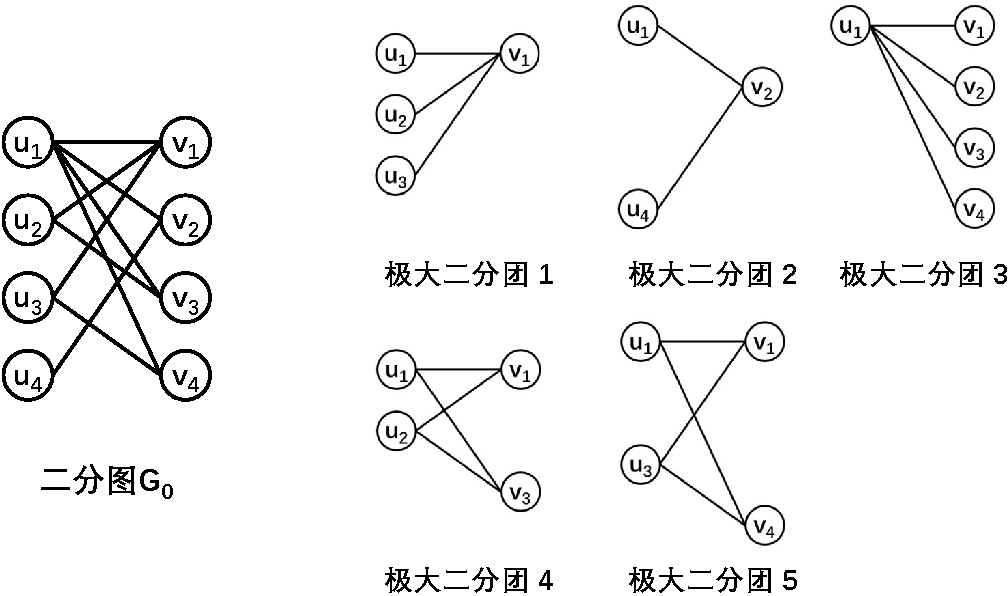
\includegraphics[width=0.7\linewidth]{eg_definition}
  \vspace{0.1 in}
  \caption{二分图中的极大二分团枚举问题示例}
  \label{fig:eg_definition}
\end{figure}

\begin{example}
  图~\ref{fig:eg_definition}给出了一个二分图中的极大二分团枚举问题的示例。其中左图是一个具有8个顶点,9条边的二分图$G_0$,右图展示了二分图中的全部极大二分团,共5个。极大二分团枚举问题即无重复、无遗漏地枚举二分图$G_0$中的全部5个极大二分团。
  
\end{example}

考虑到现有方法在处理大规模二分图时效率低下,本研究从\emph{剪枝能力} 、 \emph{数据结构} 和 \emph{并行实现}等方面入手,探索\textbf{在大规模二分图场景下的高效极大二分团枚举方法}。



% 探索在大规模二分图中高效解决极大二分团枚举问题的方法成为一项重要的研究课题。


\subsection{基本求解方法}
\label{subsec:baseline}
  
  在本节中,我们详细描述了主流的基于集合枚举树的极大二分团问题基本求解方法。我们首先介绍了极大二分团问题中的集合枚举树的定义,接着给出了基于该集合枚举树的极大二分团枚举基本算法,最后分析了该算法的复杂度。

\subsubsection{集合枚举树介绍}
\label{subsec:se}

\begin{figure} [ht]
  % \vspace{0.1 in}
  \centering
  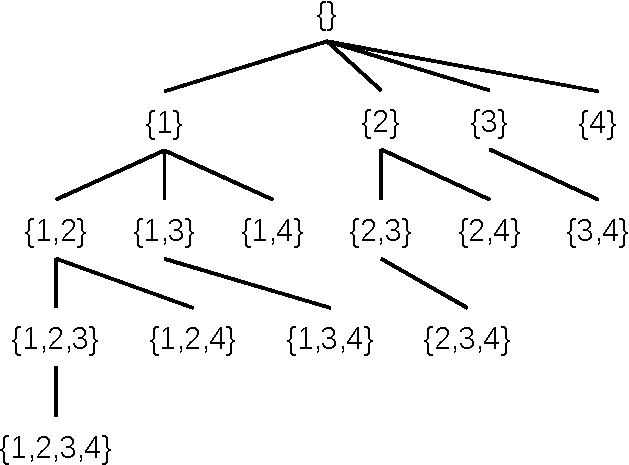
\includegraphics[width=0.45\linewidth]{se_naive}
  \vspace{0.1 in}
  \caption{对于集合$P\{1,2,3,4\}$的集合枚举树}
  \label{fig:se_naive}
\end{figure}


\textbf{集合枚举树}(Set Enumeration Tree, SE tree)是一种用于有序地枚举特定集合全部子集的数据结构,即枚举该集合的幂集~\cite{SEtree92}。它为解决搜索空间为特定集合幂集的子集的问题提供了一种完整且无冗余的搜索技术。具体而言,集合枚举树如图~\ref{fig:se_naive} 所示,根节点表示空集,每个节点对应一个子集,其子节点代表在该子集基础上添加一个新元素所得到的子集。对于二分图中的极大二分团枚举问题而言,每个二分团的集合$R$即为二分图中集合$V$的一个独特子集。因此,通过引入集合枚举树可以无重复、无遗漏地枚举全部可能的极大二分团,进而有效地求解极大二分团枚举问题。

对于应用于极大二分团枚举问题的集合枚举树,我们从以下三个角度对其进行了规范化描述:

\begin{itemize}
  \item 节点结构:每个树节点为一个三元组$(L,R,C)$。在一个二分图$G(U,V,E)$,集合$L$是集合$U$的子集,集合$R$和集合$C$是集合$V$的两个不相交子集。集合$L$和$R$构成一个二分团,其中集合$L$包含左部顶点,集合$R$包含右部顶点。集合$C$包含用于扩展集合$R$的候选顶点。
  \item 节点生成:枚举树从根节点$(U,\emptyset,V)$ 开始遍历。对于当前节点$(L,R,C)$,枚举树按顺序访问集合$C$中的每个候选顶点$v'$以生成一个新的节点$(L',R',C')$。集合$L'$包含集合$L$和集合$N(v')$中的共同顶点。集合$R'$包含集合$R$中的顶点、顶点$v'$以及集合$C$中与集合$L'$内顶点均相连且未被访问的顶点。集合$C'$包含集合$C$中与集合$L'$内顶点部分相连的且未被访问的顶点。
  \item 节点检查:当且仅当集合$L'$的共同邻居等于集合$R'$, 即$\Gamma(L')=R'$时,节点$(L',R',C')$通过节点检查,输出一个极大二分团。
\end{itemize}

此外,一些研究~\cite{iMBEA14,ooMBE22}在每个枚举节点中额外引入集合$Q$作为辅助节点检查的工具,构成四元组$(L,R,C,Q)$。其中集合$Q$于存储已访问的候选顶点,以帮助检查节点是否对应非极大二分团。具体而言,当集合$Q$中存在任意一个顶点$v_q$,并且它的邻居包含了集合$L$中的所有顶点时,根据定义~\ref{def:mb}我们可以推断当前节点对应的二分团$(L,R)$可以添加顶点$v_q$构成新的二分团,即$(L, R\cup\{v_q\})$,从而我们可以判定当前节点对应一个非极大二分团。然而,使用集合$Q$需要额外的存储和计算开销。幸运的是,我们观察到可以通过访问$L$中的任意顶点$u_l$的邻居$N(u_l)$来高效地替代集合$Q$的作用。具体而言,当集合$N(u_l)$中存在一个不在$R$集合中的顶点$v^*$,并且它的邻居包含了集合$L$中的所有顶点时,我们可以推断当前节点对应的二分团$(L,R)$可以添加顶点$v^*$构成新的二分团,从而判定当前节点对应一个非极大二分团。因此,在枚举树的介绍和相关算法中,我们不再引入集合$Q$。

\subsubsection{基于集合枚举树的极大二分团枚举基本算法}
\label{subsec:algorithm}
  结合上一节对集合枚举树的定义与描述,我们给出了基于集合枚举树的极大二分团枚举基本算法。

\begin{algorithm}[H]
    \begin{algorithmic}[1]
        \normalsize
        \REQUIRE 二分图 $G(U,V,E)$
        \ENSURE 所有极大二分团
        
        \renewcommand{\algorithmicwhile}{\textbf{procedure}}
        \renewcommand{\algorithmicdo}{\textbf{:}}


        \STATE \textsf{biclique\_search\_basic}$(U,\emptyset,V)$;
        \WHILE{\textsf{biclique\_search\_basic}$(L,R,C)$}
        \renewcommand{\algorithmicdo}{\textbf{do}}
          \FOR{$v' \in C$}
            \STATE $L' \leftarrow L \cap N(v')$; $R'\leftarrow R$; $C' \leftarrow \emptyset$;
            \FOR{$v_c \in C$}
              \IF{$L' \cap N(v_c) = L'$}
                \STATE $R' \leftarrow R' \cup \{v_c\}$;
              \ELSIF{$L' \cap N(v_c) \neq \emptyset$}
                \STATE $C' \leftarrow C' \cup \{v_c\}$;
              \ENDIF
            \ENDFOR
            \IF{$\Gamma(L') = R'$}
              \STATE 输出极大二分团$(L', R')$;
              \STATE \textsf{biclique\_search\_basic}$(L',R',C')$;
            \ENDIF
            \STATE $C \leftarrow C \setminus \{v'\}; $
          \ENDFOR

        \ENDWHILE

    \end{algorithmic}
    \caption{基于集合枚举树的极大二分团枚举算法}
    \label{alg:se_mbe}
\end{algorithm}

算法~\ref{alg:se_mbe}总结了基于集合枚举树的极大二分团枚举算法的基本枚举过程。具体而言,该算法从根节点$(U,\emptyset,V)$开始,递归地调用\textsf{biclique\_search\_basic}过程 (第1行)。过程\textsf{biclique\_search\_basic}接收一个枚举树节点作为输入,即该节点对应的集合$L$,$R$和$C$ (第2行)。在处理当前枚举节点时,该过程会逐个遍历$C$中的顶点$v'$ (第3行),然后根据集合枚举树的节点生成规则生成新节点$(L',R',C')$ (第4-11行)。随后,过程按照节点检查规则对新生成的节点$(L',R',C')$进行检查 (第12行)。如果该节点对应一个极大二分团,则输出该二分团 (第13行),并递归地调用过程\textsf{biclique\_search\_basic}以节点$(L',R',C')$为根节点继续探索子枚举树 (第14行);否则,我们知道该节点对应非极大二分团,跳过该节点。为保证$C$中的顶点都未被访问,过程会及时从$C$中移除已访问的顶点$v'$ (第16行)。我们用下面的例子对该算法进行说明。


\begin{figure} [ht]
  \vspace{0.1 in}
  \centering
  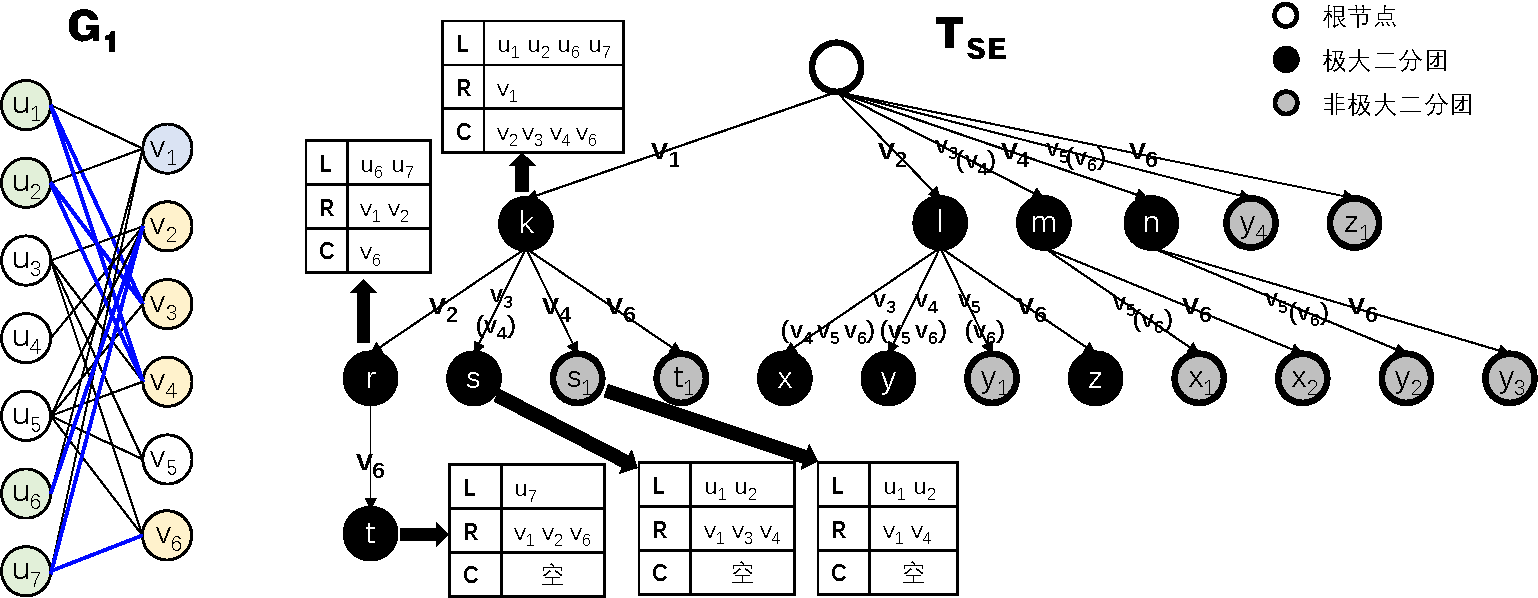
\includegraphics[width=0.98\linewidth]{se_mbea}
  \vspace{0.1 in}
  \caption{算法~\ref{alg:se_mbe}在二分图$G_1$上的集合枚举树}
  \label{fig:se_mbea}
\end{figure}

\begin{example}
  \label{example:se}
  图~\ref{fig:se_mbea}展示了算法~\ref{alg:se_mbe}在二分图$G_1$上的集合枚举树$T_{SE}$。
  \footnote{为了方便比较,全文中具有相同字母标识的节点在枚举树中共享相同的集合$L$,只有没有下标的节点会输出极大二分团。例如,节点$s$和节点$s_1$具有相同的集合$L$,但只有节点$s$会输出一个极大二分团。我们使用集合的下标来表示该集合隶属于哪个节点。例如$L_s$表示节点$s$的集合$L$。 
}
我们从根节点开始,通过深度优先搜索逐个遍历候选顶点,递归地搜索子空间。首先,我们通过遍历顶点$v_1$生成节点$k$。按照算法~\ref{alg:se_mbe}中第4-11行的计算方法,我们可以计算得到$L_k=N(v_1)=\{u_1, u_2, u_6, u_7\}$,$R_k=\{v_1\}$,$C_k=\{v_2,v_3,v_4,v_6\}$。根据节点检查规则,因为$\Gamma(L_{k}) = \{v_1\} = R_{k}$,所以节点$k$输出一个极大二分团并继续探索以节点$k$为根节点的子枚举树。为便于观察,我们在图$G_1$中标记了节点$k$中的顶点,即$L_k$,$R_k$和$C_k$中的全部顶点,并标出了集合$L_k$与集合$C_k$之间的边。

接下来,节点$k$遍历顶点$v_2$生成节点$r$。同理,我们可以计算得到$L_{r} = N(v_2) \cap L_{k} 
= \{u_3, u_4, u_5, u_6, u_7\} \cap \{u_1, u_2, u_6, u_7\} = \{u_6, u_7\}$, $R_{r} = R_{k} \cup (C_{k} \cap \Gamma(L_{r})) = \{v_1\} \cup (\{v_2, v_3, v_4, v_5\} \cap \{v_1, v_2\}) = \{v_1, v_2\}$。集合$C_{r}$中仅包含顶点 $v_6$,因为顶点$v_3$, $v_4$和 $v_5$不与集合$L$中的任何顶点相连。

继续这个过程,我们可以计算得到节点$s$以及节点$s_1$。节点$s$对应二分团$(\{u_1, u_2\},$ $\{v_1, v_3, v_4\})$,节点$s_1$对应二分团 $(\{u_1, u_2\}, \{v_1, v_4\})$。根据节点检查规则,因为$\Gamma(L_{s_1}) = \{v_1, v_3, v_4\} \neq R_{s_1} = \{v_1, v_4\}$,所以节点$s_1$对应一个非极大二分团。具体地,与节点$s$相比,节点$s_1$不能用$v_3$来扩展该节点中的集合$R_{s_1}$。这是因为在生成节点$s_1$时,根据深度优先搜索的规则,顶点$v_3$已被访问并用于生成节点$s$。因此,在节点检查之后,我们删除了节点$s_1$。同理,其他节点可以类似地生成。

\end{example}

在算法~\ref{alg:se_mbe}的基础上,现有的基于枚举树的极大二分团枚举算法的优化方法主要包括改变节点候选顶点的遍历顺序~\cite{minel06,iMBEA14,PMBE20,ooMBE22}、设计剪枝方法以提前裁剪产生非极大二分团的节点~\cite{iMBEA14,PMBE20,ooMBE22},以及并行优化~\cite{mapreduceMBE16,parMBE19}。在~\ref{sec:opt}节中,我们将对上述优化方法进行详细说明,并介绍它们在实际应用中的效果。

\subsubsection{算法复杂度分析}
\label{subsec:baseline_analysis}

结合算法伪代码,我们从时间复杂度和空间复杂度两个方面对算法~\ref{alg:se_mbe}进行分析。

\textbf{时间复杂度:} 我们首先分析枚举树中每个节点的计算时间,随后分析枚举树中的枚举节点数量,最终得到算法~\ref{alg:se_mbe}的时间复杂度。平均而言,对于每个节点$(L',R',C')$的计算包括节点生成(第4-11行)和节点检查(第12行)两个部分。由于集合$C$中最多包含$|V|$个顶点,且每个顶点的集合交集运算需要$O(\Delta(V))$的时间,因此节点生成过程的时间复杂度为$O(|V|\Delta(V))$。而节点检查过程中,我们可以通过只访问二分图中的每条边一次来获取$\Gamma(L')$的值,因此节点检查的时间复杂度为$O(|E|)$(或$O(|V|\Delta_{avg}(V))$)。综上,每个节点的计算时间为$O(|V|\Delta(V))$。为了量化算法的计算时间,我们用$\beta$来表示枚举树中节点的数量。最终,算法的时间复杂度为$O(|V|\Delta(V)\beta)$。

\textbf{空间复杂度:} 由于算法~\ref{alg:se_mbe}按照深度优先的方式进行搜索,我们可以对枚举树中每个节点占用的空间进行分析,并结合枚举树的高度以及输入二分图所占用的空间,得到算法的空间复杂度。对于每个节点$(L',R',C')$,集合$L'$最多包含$\Delta(V)$个顶点,集合$R'$和$C'$最多包含$|V|$个顶点。在二分图中,集合$V$内顶点的数量通常远高于任何单个顶点的度数,因此每个节点的空间开销为$O(\Delta(V)+|V|)=O(|V|)$。在递归过程中,节点的集合$L$内的顶点数量不断减少,因此我们可以确定枚举树的高度为$O(\Delta(V))$。考虑到二分图$G(U,V,E)$需要占用$O(|U|+|V|+|E|)=O(|E|)$的空间,最终算法的空间复杂度为$O(|E|+|V|\Delta(V))$。




\section{国内外研究现状}
\label{sec:related}

作为图论中的基础问题,关于极大二分团枚举问题的研究最早可追溯到1962年~\cite{MBE62}。在过去的几十年中,国内外学者对二分图中的极大二分团枚举问题进行了深入的研究,并取得了一系列重要的成果。

\begin{figure} [H]
  \centering
  \vspace{0.2in}
  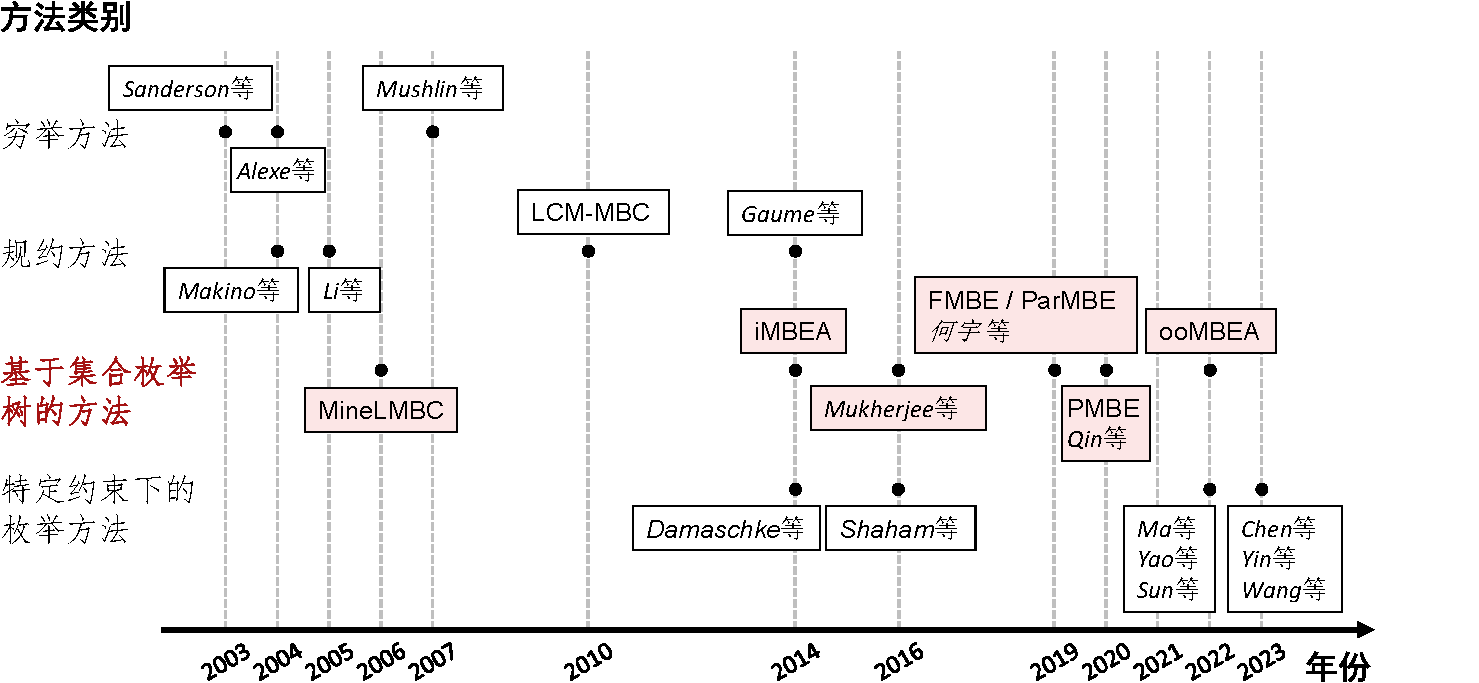
\includegraphics[width=0.98\linewidth]{related_work}
  \vspace{0.1in}
  \caption{极大二分团枚举领域国内外研究情况梳理}
  \label{fig:related_work}
\end{figure}

我们在图~\ref{fig:related_work}中对国内外相关研究进行了梳理和总结,将其分为四类。早期的研究主要采用穷举方法和规约方法,而当前的主流工作采用基于集合枚举树的方法。同时,近期的研究涉及到特定约束下的枚举方法。接下来,我们将详细介绍这四类方法。

% 我们在图~\ref{fig:related_work}中梳理并总结了国内外研究现状,将相关研究工作分为四类。早期的研究方法主要包括穷举方法和规约方法,目前的主流极大二分团枚举方法基于集合枚举树的方法实现,同时,近期的相关工作属于变种,开始研究特定约束下的二分团枚举方法,随后,我们对这四类方法进行详细说明。
% 对国内外的研究情况进行了梳理与总结。从图中可以得知,基于集合枚举树的方法目前是解决通用极大二分团枚举问题的主流方法。目前已有的极大二分团枚举方法可以归为以下四个大类:

\subsection{穷举方法}

解决极大二分团枚举问题的一种直观方法是使用穷举法生成并存储所有可能的二分团,然后对这些二分团进行极大性检测。早期工作以此观察为基础,提出了关于极大二分团枚举问题的暴力穷举求解方法。Sanderson等人提出了一种迭代算法,逐步构建出全部可能的二分团~\cite{exhaust03}。具体而言,该算法首先选取二分图中一个顶点集中的单一顶点作为初始二分团。然后,它遍历其他顶点,逐一将其加入到当前的二分团中构成新的二分团,并对所得的新的二分团进行极大性检测。随后,Alexe等人提出了一种共识算法,用于生成极大二分团。该算法将每个顶点及其邻居作为初始候选二分团,并通过不断进行共识分析来扩展新的候选二分团~\cite{MICA04}。在生成的新二分团中,还进行判断以确保其为极大二分团且没有重复。整个过程会持续进行,直到候选二分团集合不再增加。此外,Mushlin等人利用集合扩展操作构建二分团,并利用哈希表进行极大性检测。他们引入了评价指标,以支持在枚举过程中对二分团的优先级进行排序~\cite{exhaust07}。尽管这些方法能够解决极大二分团枚举问题,但它们没有充分考虑搜索空间的剪枝优化,因此在计算过程中不可避免地会产生大量非极大二分团,导致计算和存储开销增加。同时,由于时间复杂度较高,这些方法无法应用于规模较大的二分图上的极大二分团枚举问题的求解。

\subsection{规约方法}

考虑到极大二分团枚举问题和其他问题的联系,学者们尝试将二分图中的极大团枚举问题规约到其他问题,并用其他问题中的已有方法进行求解。(1) 规约到极大团枚举问题。Makino等人观察到二分图上的极大二分团枚举问题可以通过图膨胀的方式映射到通用图上的极大团枚举问题进行求解~\cite{Makino04}。具体而言,他们将二分图中的每个顶点集合内的任意两个顶点添加一条边,从而膨胀原二分图中的每个极大二分团,使其对应于膨胀后通用图中的一个极大团。通过这种方式,二分图上的极大二分团枚举问题可以被等价地转化为通用图上的极大团枚举问题。然而,需要注意的是,尽管通用图上的极大团枚举问题已经在学术界得到广泛研究,并存在一些有效的极大团枚举方法~\cite{MCEparallel20,MCE20,MCE22,MCE-GPU21,MCE-22},但直接应用这些方法并不实用。这是因为图的膨胀会引入大量的新边,从而导致计算难度的增加,并严重影响了计算性能。(2) 规约到闭频繁项集挖掘问题。Zaki等人注意到事务数据库中的闭频繁项集与二分图中的极大二分团存在一一对应的关系~\cite{FCIM98}。基于这个对应关系,Li等人指出了数据挖掘领域中一些经典算法对于极大二分团枚举问题的解决具有帮助作用~\cite{correspondence05},例如FPclose~\cite{fpclose04}和LCM~\cite{lcm04}等算法。通过计算闭频繁项集集,可以得到极大二分团中的一个顶点集合,进而计算另一个顶点集合以构成二分团。Li等人还在LCM算法的基础上提出了LCM-MBC算法来进行极大二分团枚举~\cite{lcmmbc07}。然而,对于闭频繁项集挖掘算法而言,在大规模事务性数据库中将支持度设置为1进行闭频繁项集挖掘是非常困难的~\cite{iMBEA14}。(3)规约到形式概念分析问题。Gaume等人指出二分图中的极大二分团与形式概念分析问题中的形式概念存在平行关系~\cite{fcambe10}。因此,现有的形式概念分析相关的工作~\cite{FCA15,FCA21,FCA22}可以用于极大二分团枚举问题的求解。然而,形式概念分析相关的工作主要在二进制数据上展开~\cite{FCA15},即源数据通过位图方式存储并以位运算的方式开展计算。由于现实中的二分图是稀疏的,位图存储方式会带来大量的内存开销,这导致前沿的形式概念分析算法只能在小图上进行~\cite{FCA21,FCA22},在大规模二分图中会带来内存超过限制的问题。综上所述,规约方法在大规模二分图场景下是低效的。

% \begin{figure} [t]
%   \centering
%   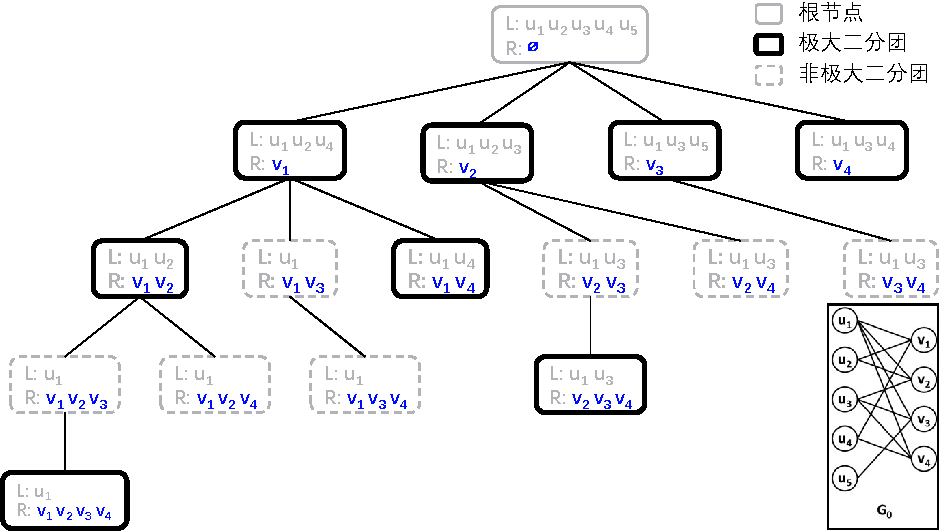
\includegraphics[width=0.62\linewidth]{se_tree}
%   \caption{极大二分团枚举算法中的集合枚举树}
%   \label{fig:se}

% \end{figure}

\subsection{基于集合枚举树的枚举方法}

如~\ref{subsec:baseline}节所述,目前,主流且高效的极大二分团枚举算法基于集合枚举树~\cite{SEtree92}的数据结构实现。
%集合枚举树是一种用于有序地枚举特定集合的所有子集的工具。 给定一个二分图$G(U, V, E)$,其中$U$和$V$表示两个不相交的顶点集合,$E$表示边集合,$E \subseteq U \times V$。该类枚举算法首先利用集合枚举树生成集合$V$的全部子集,然后将每个集合$V$的子集扩展成二分团,并输出其中的全部极大二分团。图~\ref{fig:se}展示了一棵用于极大二分团枚举的集合枚举树。集合枚举树首先将集合$V$的全部子集无重复地生成到每个树节点的集合$R$中(标记为蓝色),然后每个节点将所有与$R$内顶点完全相连的顶点作为顶点的集合$L$,最后枚举其中所有的极大二分团$(L,R)$。
2006年,Liu等人提出MineLMBC算法~\cite{minel06},首次引入集合枚举树,采用分治法求解极大二分团枚举问题。此后,基于枚举树的极大二分团枚举方法得到了不断优化。为了减少搜索空间、提升计算效率,研究者们相继提出了不同的优化技术。Zhang等人提出iMBEA算法~\cite{iMBEA14},采用了顶点度数升序排序和排除顶点集等技术,以减少枚举时间。Das等人提出FMBE算法~\cite{parMBE19},通过主动计算顶点的二跳邻居作为候选顶点集合,加速了枚举过程。Abidi等人提出PMBE算法~\cite{PMBE20},借鉴了极大团枚举问题中的枢纽顶点思路,利用枢纽顶点进行剪枝。Chen等人提出ooMBEA算法~\cite{ooMBE22},引入了单边排序和批量枢纽顶点剪枝等技术,进一步减少了枚举时间。为了进一步提高效率,研究者们设计了并行极大二分团枚举算法。Mukherjee等人利用MapReduce框架实现了分布式极大二分团枚举算法CDFS~\cite{mapreduceMBE16}。然而,大量的跨节点通信开销导致该算法效率较低。Das等人提出多核算法ParMBE~\cite{parMBE19},但该算法的并行性受到计算核心数量的限制。此外,国内的He等人提出优化的sMBEA算法~\cite{MBEHe18,MBEchinese19},Qin等人利用栈的特性实现了EMBE算法~\cite{MBEQin20}。然而,相较于主流算法(如FMBE、PMBE、ooMBEA),这些算法存在较大的性能差距。综上所述,基于枚举树的极大二分团枚举方法
% 适合解决大规模二分图中的极大二分团枚举问题,但
仍存在较大的优化空间。

\subsection{特定约束下的枚举方法}

除了上述研究,一些学者对输入的二分图以及输出的极大二分团进行了特定的约束。Damaschke等人提出了一种输出敏感的极大二分团枚举算法~\cite{Damaschke14},该算法基于二分图中顶点度数的倾斜分布。然而,该算法对输入二分图的要求较为严格,仅适用于特定情况下的求解,无法很好地适用于一般二分图。Shaham等人提出了基于聚类的方法~\cite{Shaham16},在二分团搜索的子空间中利用蒙特卡洛方法获取随机种子并将其扩展为极大二分团。然而,这种方法只能枚举部分的极大二分团,无法覆盖所有可能的极大二分团。针对动态二分图,Ma等人提出了一种有效保持最大二分团性质的框架,该框架可以在动态变化的二分图上进行高效的极大二分团枚举~\cite{Ma22}。此外,近年来的一些研究工作定义了特殊类型的极大二分团,并对这些特殊类型的二分团进行枚举。例如,Yao等人定义了极大相似二分团~\cite{SimilarMBE22},Sun等人定义了极大平衡有符号二分团~\cite{Sun22}和最大有符号二分团~\cite{Sun23},Chen等人用多个极大二分团并集定义了二分团渗透社区~\cite{BicliqueCommunity23},Yin等人定义了极大二分团的公平性~\cite{FairMBE23},而Wang等人定义了不确定图场景下的极大二分团~\cite{MBEU23}。这些算法都基于极大二分团枚举算法,并在枚举过程中对输出进行适当的约束和限制,以适应特定的问题需求。然而,这些算法主要关注特定约束场景下的搜索空间剪枝与优化,难以用于加速传统的极大二分团枚举问题。综上所述,极大二分团枚举在这些研究中发挥着基础性作用。

% 除了上述工作外,其他研究对输入的二分图以及输出的极大二分团进行了特定的约束。Damaschke等人提出了一种输出敏感的极大二分团枚举算法~\cite{Damaschke14},该算法基于二分图中顶点度数的倾斜分布。然而,该算法对输入二分图的要求较为苛刻,只适用于特定情况下的求解,并不能很好地适用于一般二分图。Shaham等人提出基于聚类的方法~\cite{Shaham16},在二分团搜索的子空间中利用蒙特卡洛方法获取随机种子并将其扩展为极大二分团。然而,这种方法只能枚举部分的极大二分团,无法覆盖所有可能的极大二分团。针对动态二分图,Ma等人提出了一种有效保持最大二分团性质的框架,该框架可以在动态变化的二分图上进行高效的极大二分团枚举。另外,近年来的一些研究工作定义了特殊类型的极大二分团,并对这些特殊类型的二分团进行枚举。例如,Yao等人定义了极大相似二分团~\cite{SimilarMBE22},Sun等人定义了极大平衡有符号二分团~\cite{Sun22}和最大有符号二分团~\cite{Sun23},Chen等人用多个极大二分团并集定义了二分团渗透社区~\cite{BicliqueCommunity23},Yin等人定义了极大二分团的公平性~\cite{FairMBE23}以及Wang等人定义了不确定图场景下的极大二分团~\cite{MBEU23}。这些算法都是基于极大二分团枚举算法,并在枚举过程中对输出进行适当的约束和限制,以适应特定的问题需求。然而这些算法只注重在特定约束场景下的搜索空间剪枝与优化,这些方法难以用于加速传统的极大二分团枚举问题。综上所述,极大二分团枚举在这些研究中发挥着基础性作用。


\section{研究挑战}

尽管在极大二分团枚举领域已经有很多出色的工作,但是在处理大规模二分图时,已有方法的计算性能仍然有很大的提升空间。本节将指出主流的基于集合枚举树的枚举方法所面临的三个共性问题,并介绍解决这些问题所面临的具体挑战。

\subsection{搜索空间大,剪枝方法欠佳}

极大二分团枚举问题具有搜索空间大的特点。常见的图算法,如深度优先搜索~\cite{wiki-dfs}、广度优先搜索~\cite{wiki-bfs}、最小生成树~\cite{wiki-mst}、最短路径等算法~\cite{wiki-sssp},其搜索空间随着图的规模线性增长。而常见的图模式挖掘算法的目标子图往往只包含少量顶点~\cite{peregrine20,pangolin20,g2miner22,decomine22,khuzdul23,gamma23,Graphset23},例如三角计数问题中目标子图仅包含3个顶点~\cite{triangle18}。相比之下,极大二分团枚举问题的搜索空间更大,因为它随着二分图中顶点数量的指数级增长,并且目标子图(即极大二分团)中的顶点数量相对较多。为了应对搜索空间巨大的挑战,研究人员提出了各种优化技术,旨在减少搜索空间中产生非极大二分团的无效枚举节点,进而减少枚举时间。然而,由于搜索空间的规模庞大,现有的优化方法往往难以完全覆盖所有无效节点。具体而言,通过~\ref{subsec:ambea_exp_overall}节的实验,我们观察到现有的最新算法ooMBEA在Github数据集上需要检查并消除比极大二分团数量多26倍的产生非极大二分团的无效枚举节点。这些无效枚举节点带来大量的节点检查开销,严重降低了计算性能。因此,如何设计高效的剪枝方法来裁剪巨大搜索空间仍然是一个关键的挑战。


\subsection{计算不规则,单一结构低效}

极大二分团枚举问题具有计算不规则的特点。与其他图计算问题类似,在真实世界中,二分图的顶点邻居数量存在较大差异,导致每次计算涉及的顶点数量不同,即计算不规则~\cite{Irregularity12}。为了高效地解决这类问题,研究者们提出了多种存储结构来表示图的邻接关系。常用的存储结构包括位图~\cite{lcm04,lcmmbc07,FCA15,FCA21,FCA22}、邻接表~\cite{iMBEA14,PMBE20,ooMBE22}和哈希表~\cite{parMBE19}。不同的存储结构适用于不同场景。
例如,位图结构采用位运算,具有高效的计算能力,但在稀疏图场景下会占用更多的存储资源,因此适用于稠密小图;邻接表精确地存储每个顶点的邻居信息,在处理稀疏大图时占用较少的内存,但计算过程需要执行大量的比较运算,其运行时间与顶点个数成正比,会导致计算相对低效,因此适用于稀疏大图;哈希表具有灵活性和便于快速查找的特点,可以快速判断任意两个顶点之间的连接关系,但相比邻接表,它需要更多的存储空间并且访问方式更为随机。然而,目前的研究往往采用固定的数据结构来存储顶点的邻居信息,未能充分发挥不同数据结构的优势。因此,在枚举过程中如何动态选择合适的存储结构,发挥计算潜力,是一个关键挑战。



\subsection{负载不均匀,并行扩展性差}

极大二分团枚举问题具有负载不均匀的特点,限制了问题的并行扩展能力。为了进一步提高问题求解的效率,研究人员尝试设计并行算法来处理极大二分团枚举问题~\cite{mapreduceMBE16, MBEHe18, parMBE19}。这些算法将整个集合枚举树分解成多个子枚举树,然后利用分布式系统或多核CPU的大量计算资源来并行处理这些子树。然而,由于不同子枚举树的极大二分团的大小不同,导致计算负载之间存在较大差异。因此,即使有大量计算资源可用,计算任务的运行时间仍然受限于最耗时的负载。GPU作为一种专门用于并行计算的硬件设备,由于其内部拥有大量的计算单元,非常适合处理并行任务。然而,由于GPU和CPU在体系结构、内存层次结构以及编程模型等方面存在较大差异,现有的极大二分团枚举算法无法直接迁移到GPU系统中。尽管GPU被广泛用于加速相关的图算法,如极大团枚举~\cite{MCEGPUBitset13,MCEGPUdpp17,MCE-GPU21} 和图模式挖掘~\cite{g2miner22,SubgraphGpu22,Kclique22,stmatch22},但在GPU上进行极大二分团枚举问题仍然具有挑战性。具体来说,GPU上的极大二分团枚举问题面临着与极大二分团枚举问题类似的性能问题,许绍显等人指出GPU加速极大团枚举问题的研究极为有限~\cite{MCEreview22}。即使最新的基于GPU的极大团枚举算法GBK~\cite{MCE-GPU21} 获得较低的性能,也仅与CPU上的单线程串行算法相当。GPU上的子图枚举问题中被枚举子图通常仅包含少量顶点,而极大二分团通常包含大量顶点,因此带来更加严重的负载不均问题,导致最新的基于GPU的GPM框架G$^2$Miner~\cite{g2miner22}与GraphSet~\cite{Graphset23}中的优化无法直接解决GPU上进行极大二分团枚举面临的负载不均匀问题。因此,如何实现负载均衡并突破现有算法在并行能力方面的限制,设计基于GPU的并行极大二分团枚举方法是一个重要挑战。

\section{研究内容}



针对上一节提到的三个方面的研究挑战,本文分别从这三个角度对大规模二分图场景下的极大二分团枚举问题进行深入研究,并相应地提出了三个独立高效的算法,相较现有方法均有明显的性能提升。具体研究内容如下:

第一,针对现有剪枝方法效率低下的问题,本文提出了激进的极大二分团枚举算法AMBEA(Aggressive MBE Algorithm)。我们观察到,现有算法为了保证正确性,仅允许使用部分顶点生成新的枚举节点,导致产生大量非极大二分团;同时,现有的剪枝方法总是在节点检查后被动执行,限制了剪枝能力。因此,我们设计了以下两种方法:(1)激进的集合枚举树,允许使用全部顶点生成新的枚举节点,并利用父子节点间的联系消除枚举树中的重复二分团;(2)激进的顶点合并剪枝方法,在枚举节点生成的同时,主动合并具有相同局部邻居的顶点,提升剪枝效率。实验结果显示,AMBEA算法相较于其他次优的现有算法,可以压缩搜索空间9.0倍,并获得最多5.3倍的性能提升。

第二,针对现有静态数据结构低效的问题,本文提出了自适应的极大二分团枚举算法AdaMBE(Adaptive MBE)。我们观察到,现有算法在计算过程中,包含活跃顶点的计算子图在动态变化,导致冗余的内存访问和低效的集合运算性能。因此,我们设计了以下两种方法:(1)基于局部计算子图的优化方法,在该子图上完成节点生成等核心计算操作,减少了在该子图外的冗余顶点访问;(2)基于位图的动态子图方法,在小的计算子图上利用位图加速集合运算。实验结果显示,AdaMBE算法相较于其他次优的现有算法获得了最多49.7倍的性能提升,并成功应用于超过百亿极大二分团的大数据集。

第三,针对现有基于CPU的算法并行扩展性差的问题,本文提出了基于GPU的极大二分团枚举算法GMBE(GPU-based MBE)。我们观察到,将现有算法迁移到GPU上主要面临内存短缺、线程分歧和负载不均三方面问题。因此,我们设计了以下三种方法:(1)基于枚举节点重用的迭代方法,通过重用父节点内存生成子节点,避免为大量子节点动态分配内存;(2)局部邻居数量感知的剪枝方法,通过对局部邻居数量这一中间结果进行批量比较,在剪枝的同时最小化线程分歧问题;(3)负载感知的任务调度方法,通过对运行时的大任务根据枚举节点信息进行进一步拆分,实现了细粒度的负载均衡。实验结果显示,GMBE算法相比于最优并行算法获得了最多70.6倍的性能提升。




\section{本文的组织结构}

\begin{figure} [ht]
  \vspace{-0.2 in}
  \centering
  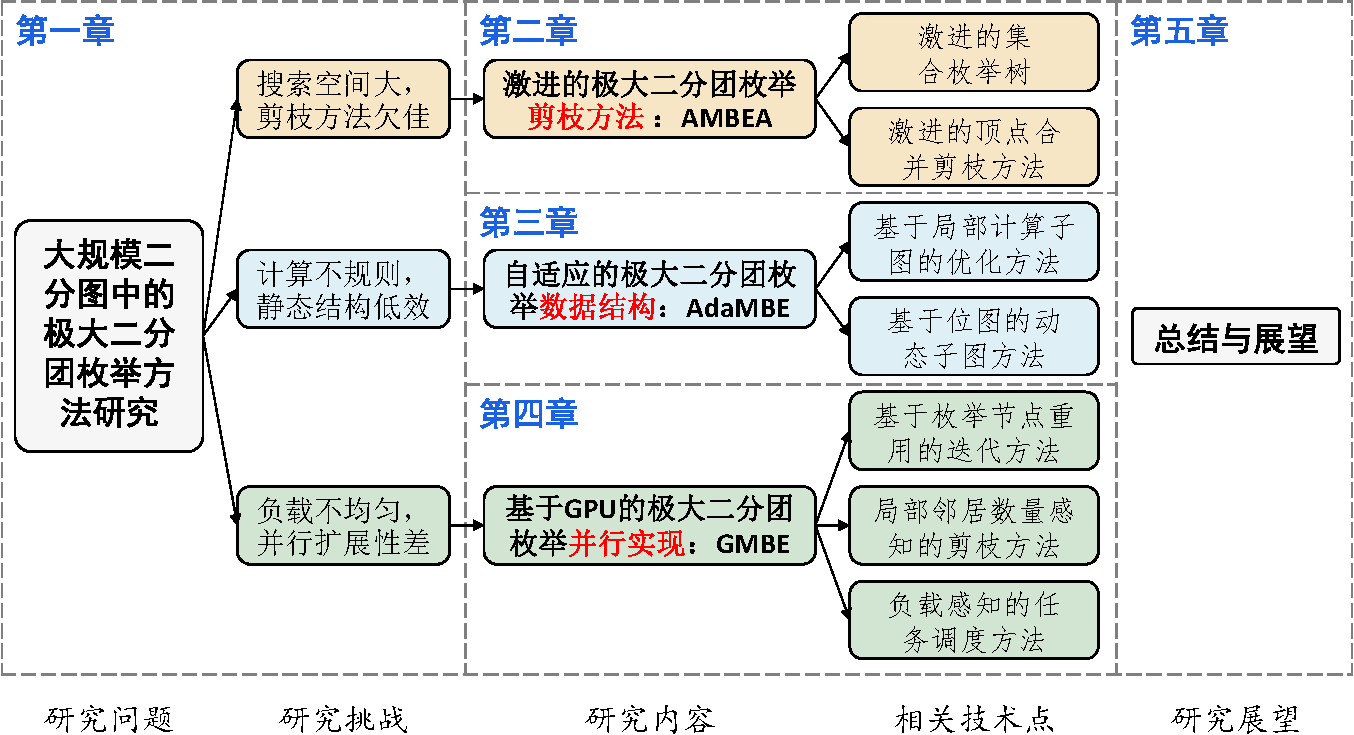
\includegraphics[width=0.82\linewidth]{outline_new}
  \vspace{-0.05 in}
  \caption{本文的组织结构图}
  \label{fig:outline}
\end{figure}

% 第一章作为绪论,介绍了研究背景、研究课题、国内外研究现状和研究挑战,并概述了本文的主要研究内容。考虑到极大二分团枚举在数据挖掘领域和图论领域中的重要应用,我们将本文的研究课题确定为在大规模二分图中的极大二分团枚举方法研究,并

图~\ref{fig:outline}展示了本文的研究内容和结构,共五个章节。
%
第一章作为绪论,首先介绍了研究背景、研究课题以及国内外的研究现状。本文主要研究大规模二分图场景下的极大二分团枚举问题。针对剪枝方法、数据结构和并行实现等三个方面的挑战,本文提出三个高效的算法,分别对应于论文的第二、第三和第四章。
%
第二章提出了AMBEA算法,主要包括激进的集合枚举树和激进的顶点合并剪枝方法两个核心技术点。通过深度优化剪枝方法,AMBEA算法在搜索空间和性能方面相较于现有最优算法有明显提升。
%
第三章提出了AdaMBE算法,主要包括基于局部计算子图的优化方法和基于位图的动态子图方法两个核心技术点。AdaMBE算法根据极大二分团枚举任务中计算子图动态变化的特点,采用自适应的数据结构,在性能上比现有算法有较大提升。
%
第四章提出了GMBE算法,主要包括基于枚举节点重用的迭代方法、局部邻居数量感知的剪枝方法以及负载感知的任务调度方法三个核心技术点。相比于现有算法只能在CPU上实现,GMBE在GPU上实现了较大幅度的性能提升。
%
第五章对全文进行总结,并展望未来的研究方向。












% 第一章介绍了大规模二分图中的极大二分团枚举问题在数据挖掘领域和图论领域中重要作用,以及国内外的相关研究工作现状。

% 第二章详细地介绍了二分图中的极大二分团枚举问题。本章首先给出问题的正式定义与相关符号定义,然后介绍了主流的基于集合枚举树的极大二分团枚举方法,最后指出现有方法现有方法在大规模二分图中进行极大二分团枚举所呈现的低效性问题,具体包含搜索空间优化、数据结构选择以及并行扩展三个方面的挑战。针对这些挑战,本文在第三至第五章分别提出三种不同的解决方案。

% 第二章介绍了激进的极大二分团枚举剪枝方法,以优化搜索空间提升枚举性能。针对现有的极大二分团枚举方法在大规模二分图中仍会产生大量非极大二分团的问题,本章提出了一种激进的集合枚举树和一种激进的顶点合并剪枝方法,并结合上述两种方法形成AMBEA算法。%实验证明,AMBEA算法在大规模二分图中的枚举性能优于现有方法,得益于其高效的剪枝性能。

% 第三章介绍了自适应的极大二分团枚举数据结构,采用混合数据结构以提升枚举性能。针对现有极大二分团枚举方法采用单一数据结构所带来的低效性问题,本章针对位图和邻接表两种数据结构分别提出了不同的计算模式,并结合这两种计算模式形成AdaMBE算法。%实验证明,基于混合数据结构的AdaMBE枚举算法比现有方法更具计算优势。

% 第四章介绍了基于GPU的极大二分团枚举并行实现,利用GPU的大量计算核心极大地缩短了枚举时间。针对现有极大二分团枚举算法只能在基于CPU的计算系统中运行且受限于计算核心数量的计算性能问题,本章提出了基于GPU的极大二分团枚举算法。针对在GPU上进行极大二分团枚举所面临的内存不足、线程分歧以及负载不均问题,本章提出了基于枚举节点重用的迭代方法、局部邻居数量感知的剪枝方法和负载感知的任务调度方法,最终形成GMBE算法。%实验证明,基于GPU的GMBE算法在性能上显著优于现有基于CPU的方法,具有更短的执行时间。

% 第五章对全文进行总结,并展望未来的研究方向。



